\pdfminorversion=4
\documentclass[aspectratio=169]{beamer}

\mode<presentation>
{
  \usetheme{default}
  \usecolortheme{default}
  \usefonttheme{default}
  \setbeamertemplate{navigation symbols}{}
  \setbeamertemplate{caption}[numbered]
  \setbeamertemplate{footline}[frame number]  % or "page number"
  \setbeamercolor{frametitle}{fg=white}
  \setbeamercolor{footline}{fg=black}
} 

\usepackage[english]{babel}
\usepackage[utf8x]{inputenc}
\usepackage{tikz}
\usepackage{courier}
\usepackage{array}
\usepackage{bold-extra}
\usepackage{minted}
\usepackage[thicklines]{cancel}
\usepackage{fancyvrb}

\xdefinecolor{dianablue}{rgb}{0.18,0.24,0.31}
\xdefinecolor{darkblue}{rgb}{0.1,0.1,0.7}
\xdefinecolor{darkgreen}{rgb}{0,0.5,0}
\xdefinecolor{darkgrey}{rgb}{0.35,0.35,0.35}
\xdefinecolor{darkorange}{rgb}{0.8,0.5,0}
\xdefinecolor{darkred}{rgb}{0.7,0,0}
\definecolor{darkgreen}{rgb}{0,0.6,0}
\definecolor{mauve}{rgb}{0.58,0,0.82}
\definecolor{darkgreen2}{rgb}{0,0.5,0}

\title[2019-10-17-pyhep-awkward]{Awkward 1.0}
\author{Jim Pivarski}
\institute{Princeton University -- IRIS-HEP}
\date{October 17, 2019}

\usetikzlibrary{shapes.callouts}

\begin{document}

\logo{\pgfputat{\pgfxy(0.11, 7.4)}{\pgfbox[right,base]{\tikz{\filldraw[fill=dianablue, draw=none] (0 cm, 0 cm) rectangle (50 cm, 1 cm);}\mbox{\hspace{-8 cm}
\includegraphics[height=1 cm]{princeton-logo-long.png}\hspace{0.1 cm}\raisebox{0.1 cm}{
\includegraphics[height=0.8 cm]{iris-hep-logo-long.png}}\hspace{0.1 cm}}}}}

\begin{frame}
  \titlepage
\end{frame}

\logo{\pgfputat{\pgfxy(0.11, 7.4)}{\pgfbox[right,base]{\tikz{\filldraw[fill=dianablue, draw=none] (0 cm, 0 cm) rectangle (50 cm, 1 cm);}\mbox{\hspace{-8 cm}
\includegraphics[height=1 cm]{princeton-logo.png}\hspace{0.1 cm}\raisebox{0.1 cm}{
\includegraphics[height=0.8 cm]{iris-hep-logo.png}}\hspace{0.1 cm}}}}}

% Uncomment these lines for an automatically generated outline.
%\begin{frame}{Outline}
%  \tableofcontents
%\end{frame}

% START START START START START START START START START START START START START

\begin{frame}{On Scientific Linux, uproot/awkward/coffea is mainstream}
\vspace{0.5 cm}
\begin{columns}
\column{1.2\linewidth}
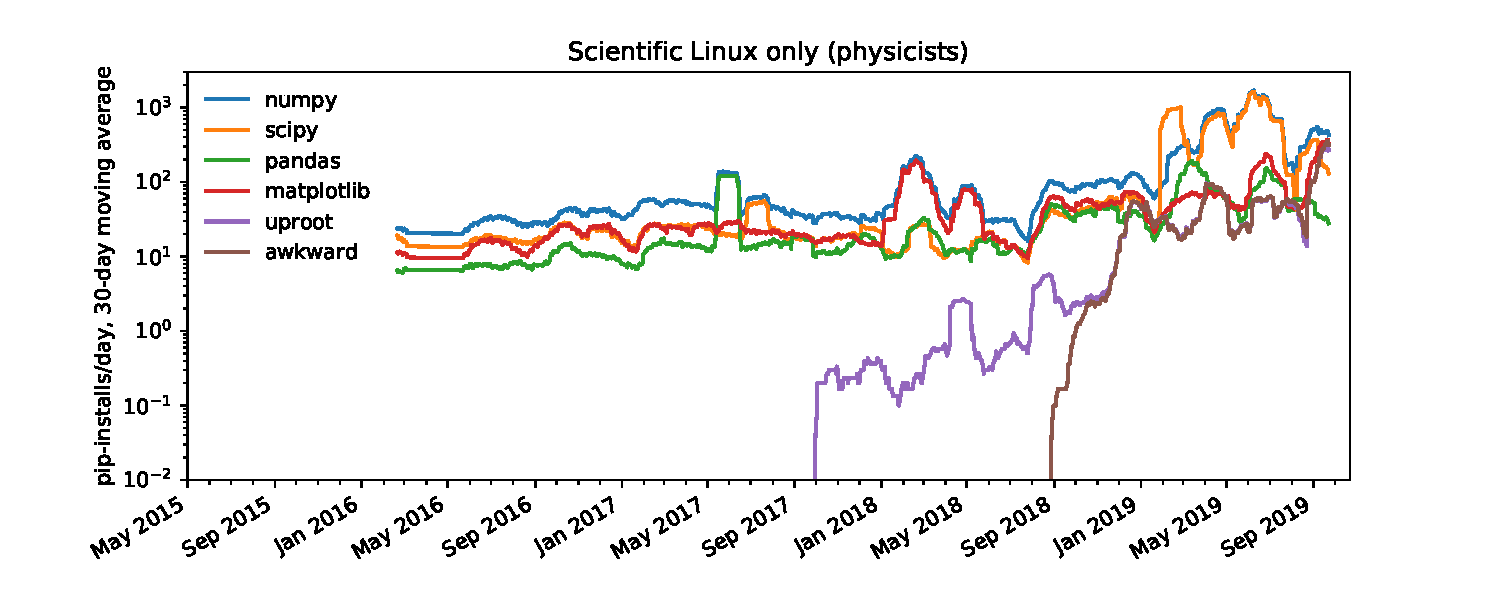
\includegraphics[width=\linewidth]{pip-scilinux-uproot.pdf}
\end{columns}
\end{frame}

\begin{frame}{But not outside of particle physics, obviously}
\vspace{0.5 cm}
\begin{columns}
\column{1.2\linewidth}
\only<1>{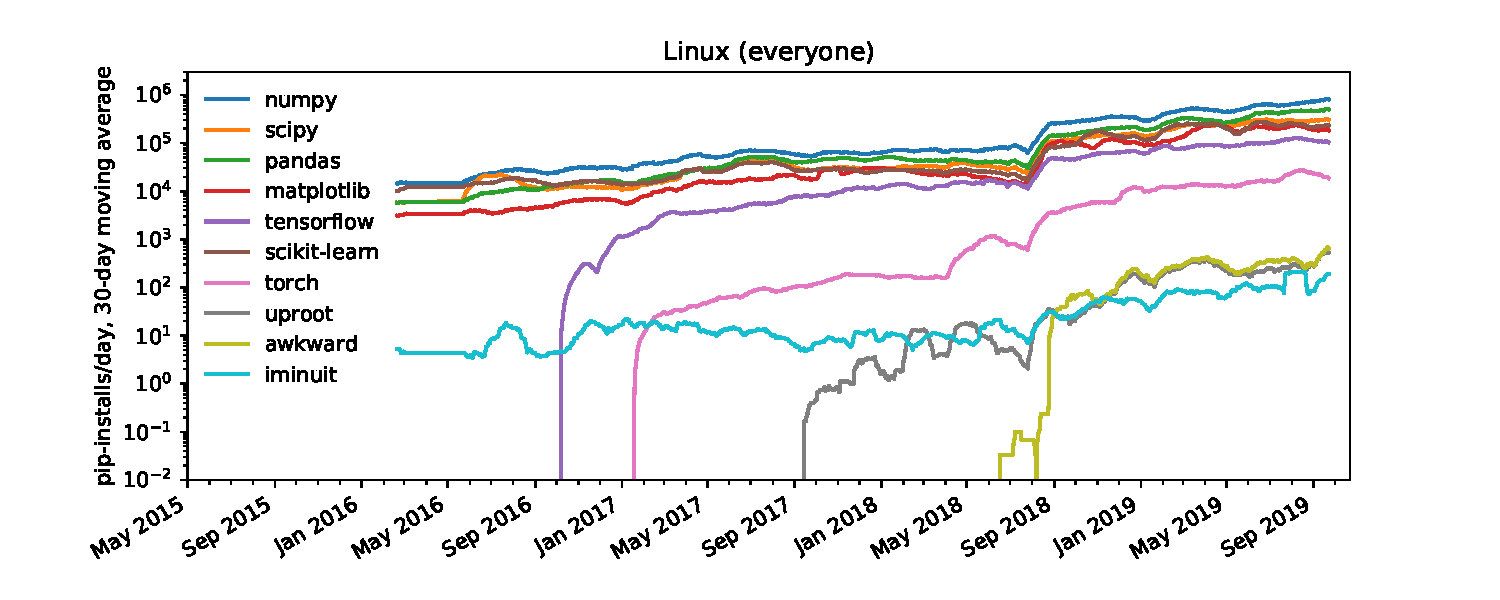
\includegraphics[width=\linewidth]{pip-linux.pdf}}\only<2>{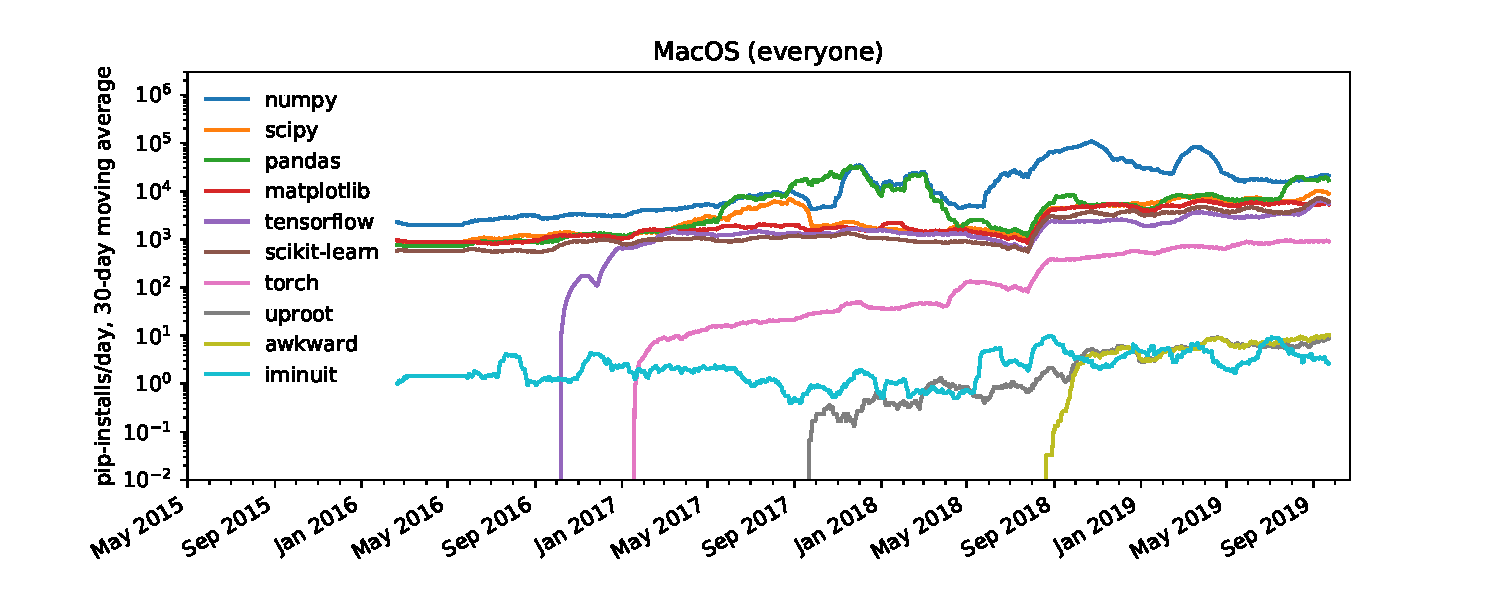
\includegraphics[width=\linewidth]{pip-macos.pdf}}\only<3>{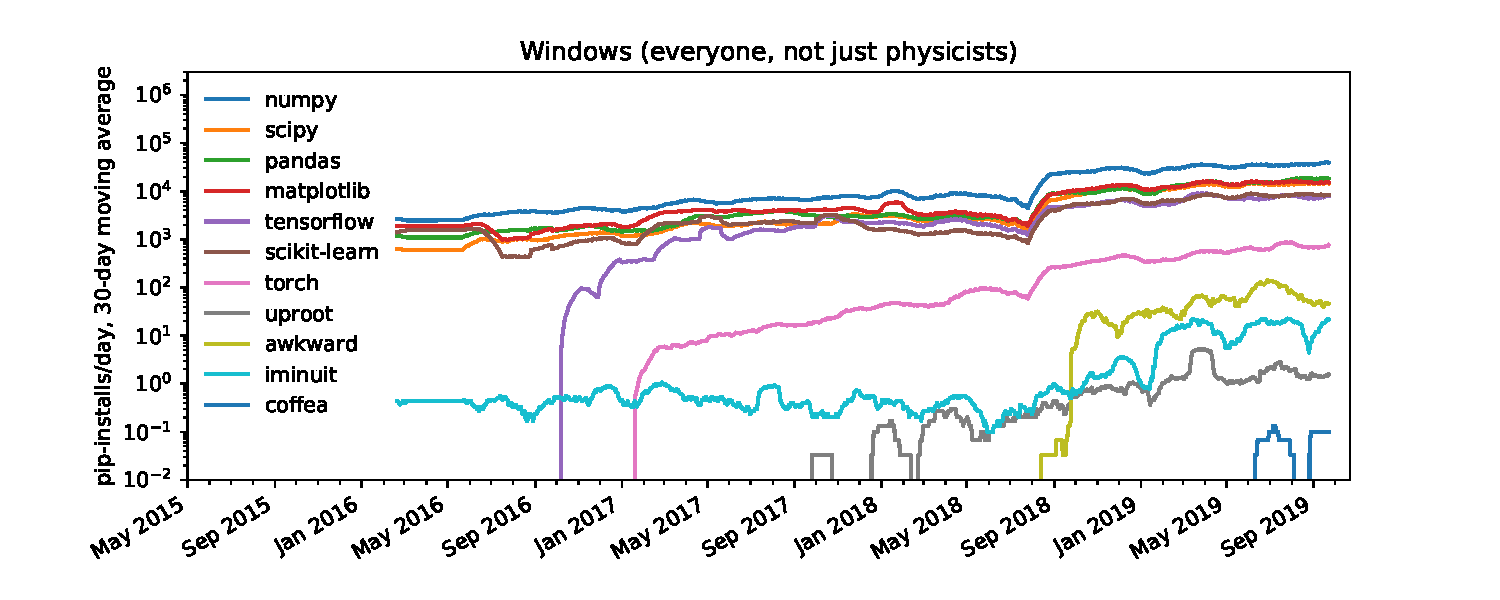
\includegraphics[width=\linewidth]{pip-windows.pdf}}
\end{columns}
\end{frame}

\begin{frame}{Uproot/Awkward maintainance is pretty much constant}
\Large
\vspace{0.75 cm}
\begin{columns}
\column{0.36\linewidth}
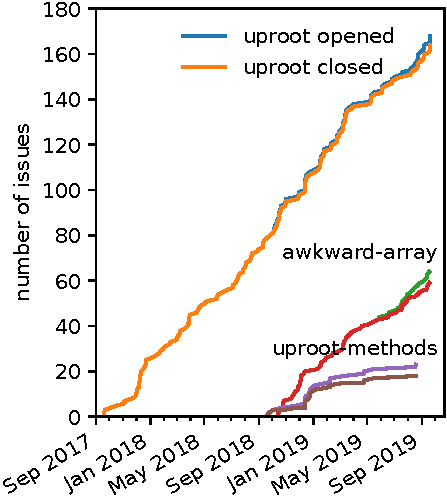
\includegraphics[width=\linewidth]{uproot-issues.pdf}

\column{0.72\linewidth}
\only<1>{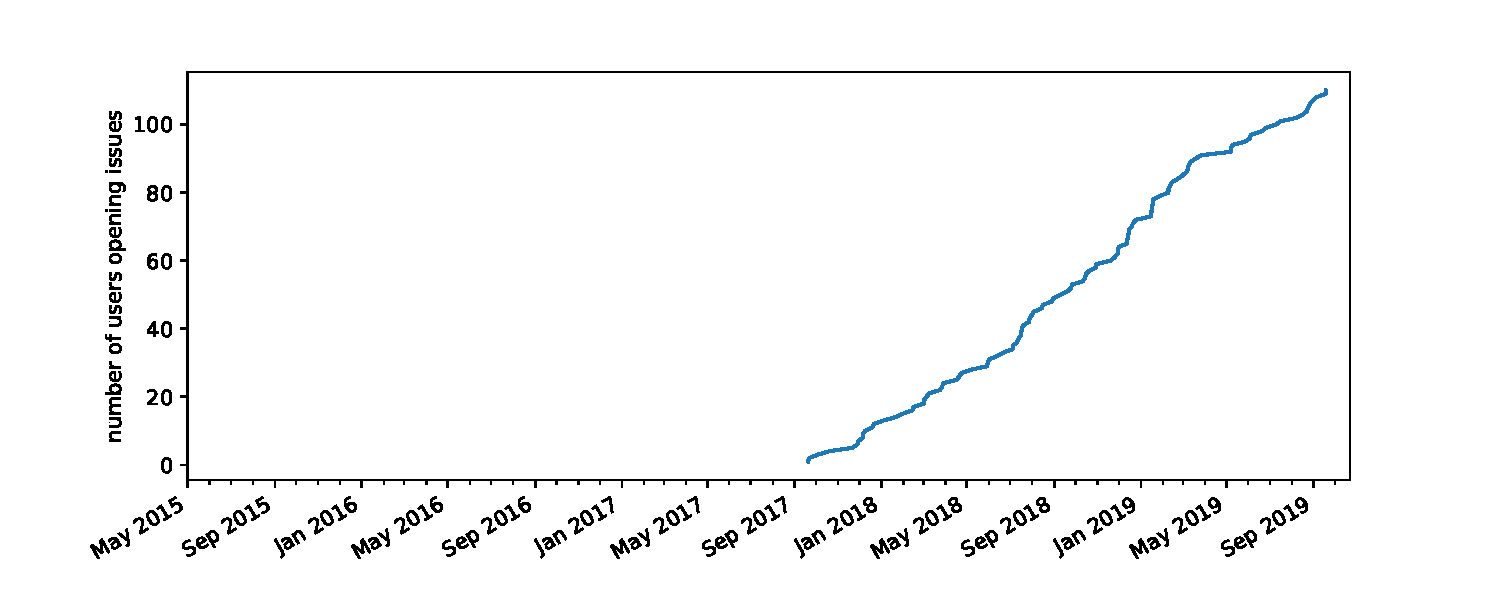
\includegraphics[width=0.5\linewidth]{uproot-users.pdf}\hfill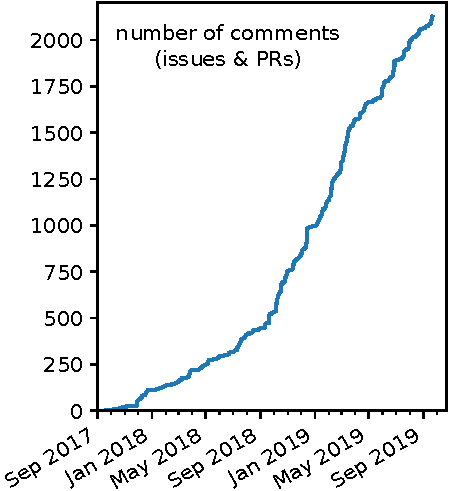
\includegraphics[width=0.5\linewidth]{uproot-comments.pdf}}\only<2->{\hfill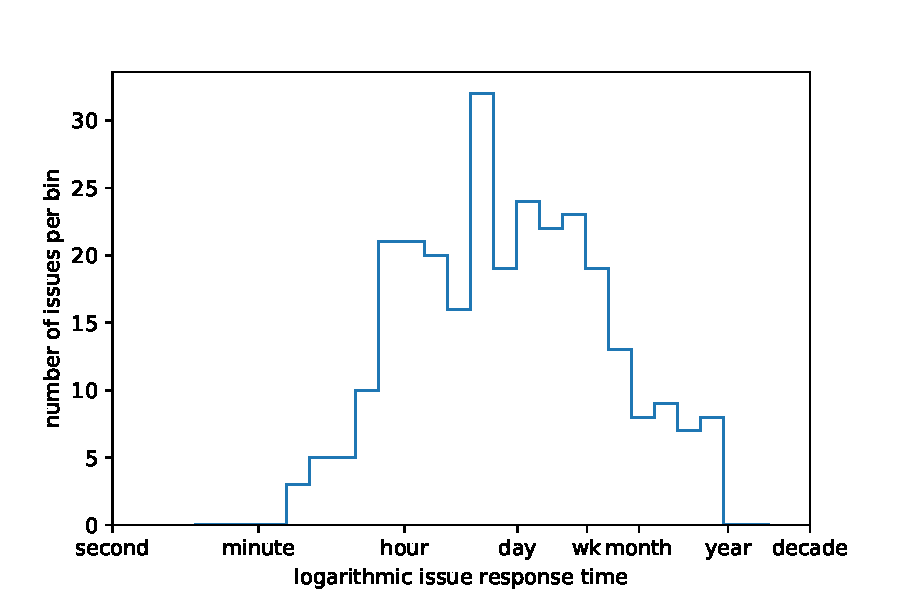
\includegraphics[width=0.45\linewidth]{uproot-response-time.pdf}\hfill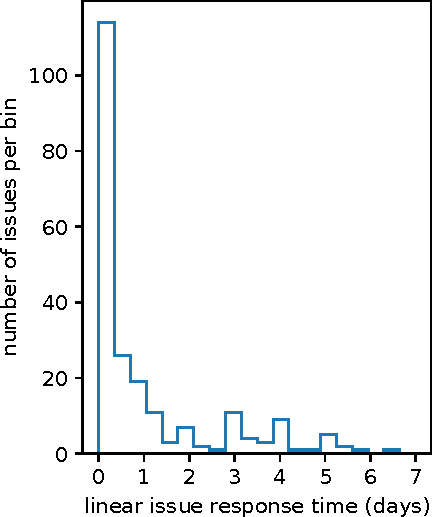
\includegraphics[width=0.45\linewidth]{uproot-response-time-linear.pdf}}
\end{columns}

\vspace{0.25 cm}
\begin{center}
\uncover<3->{The problem with GitHub issues is that once closed, they disappear.}
\end{center}
\end{frame}

\begin{frame}{Let's use StackOverflow (like most non-HEP software communities)}
\begin{center}
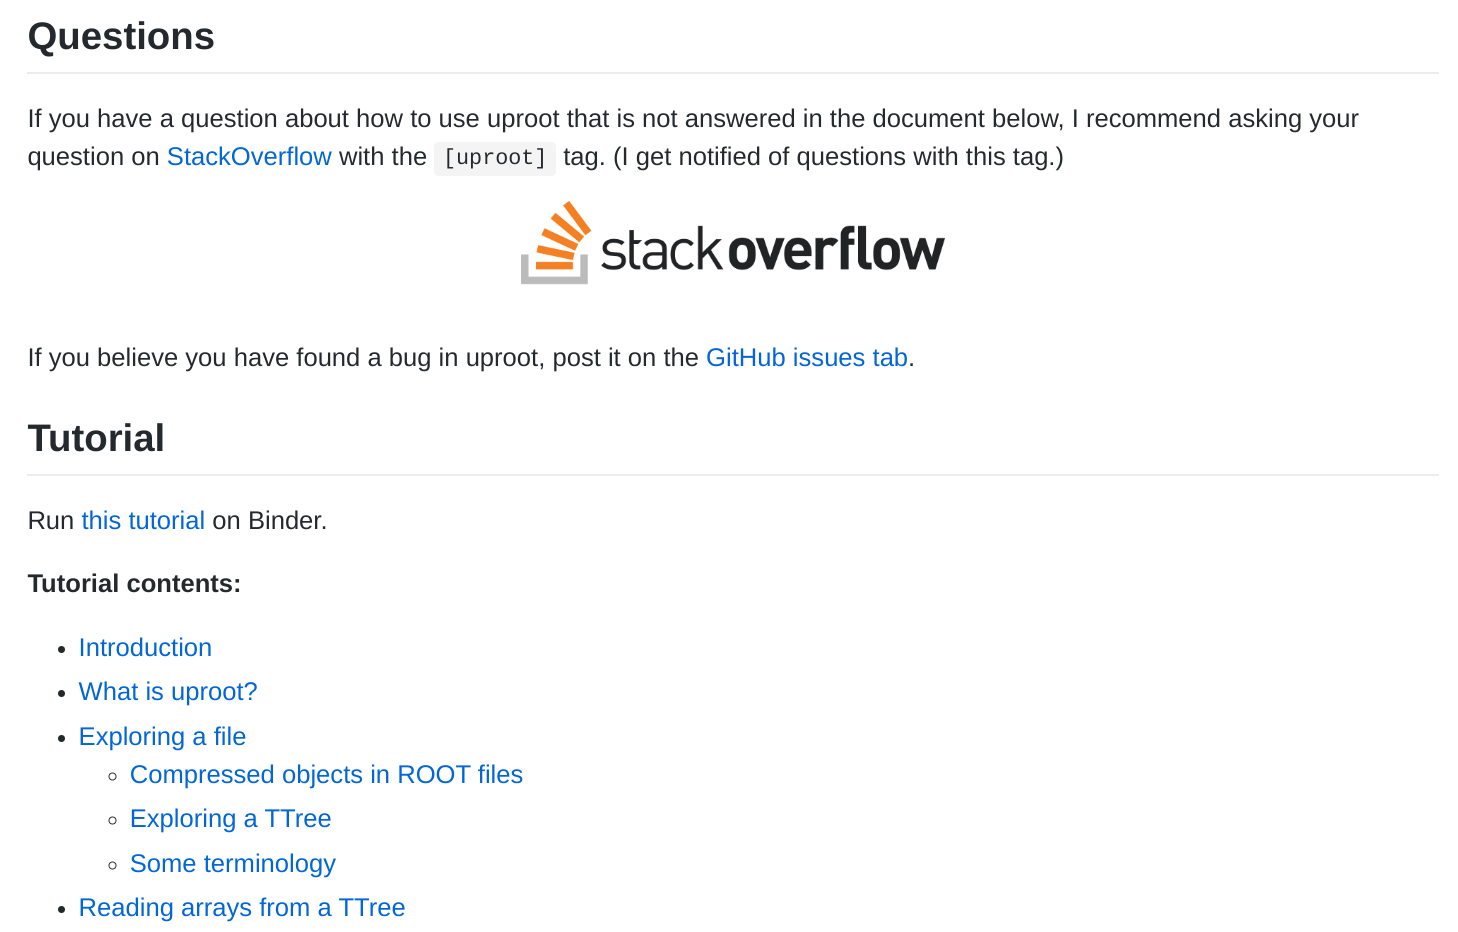
\includegraphics[width=0.88\linewidth]{uproot-stackoverflow.png}
\end{center}
\end{frame}

\begin{frame}{No, seriously, do it now.}
\vspace{0.15 cm}
\begin{columns}
\column{1.2\linewidth}
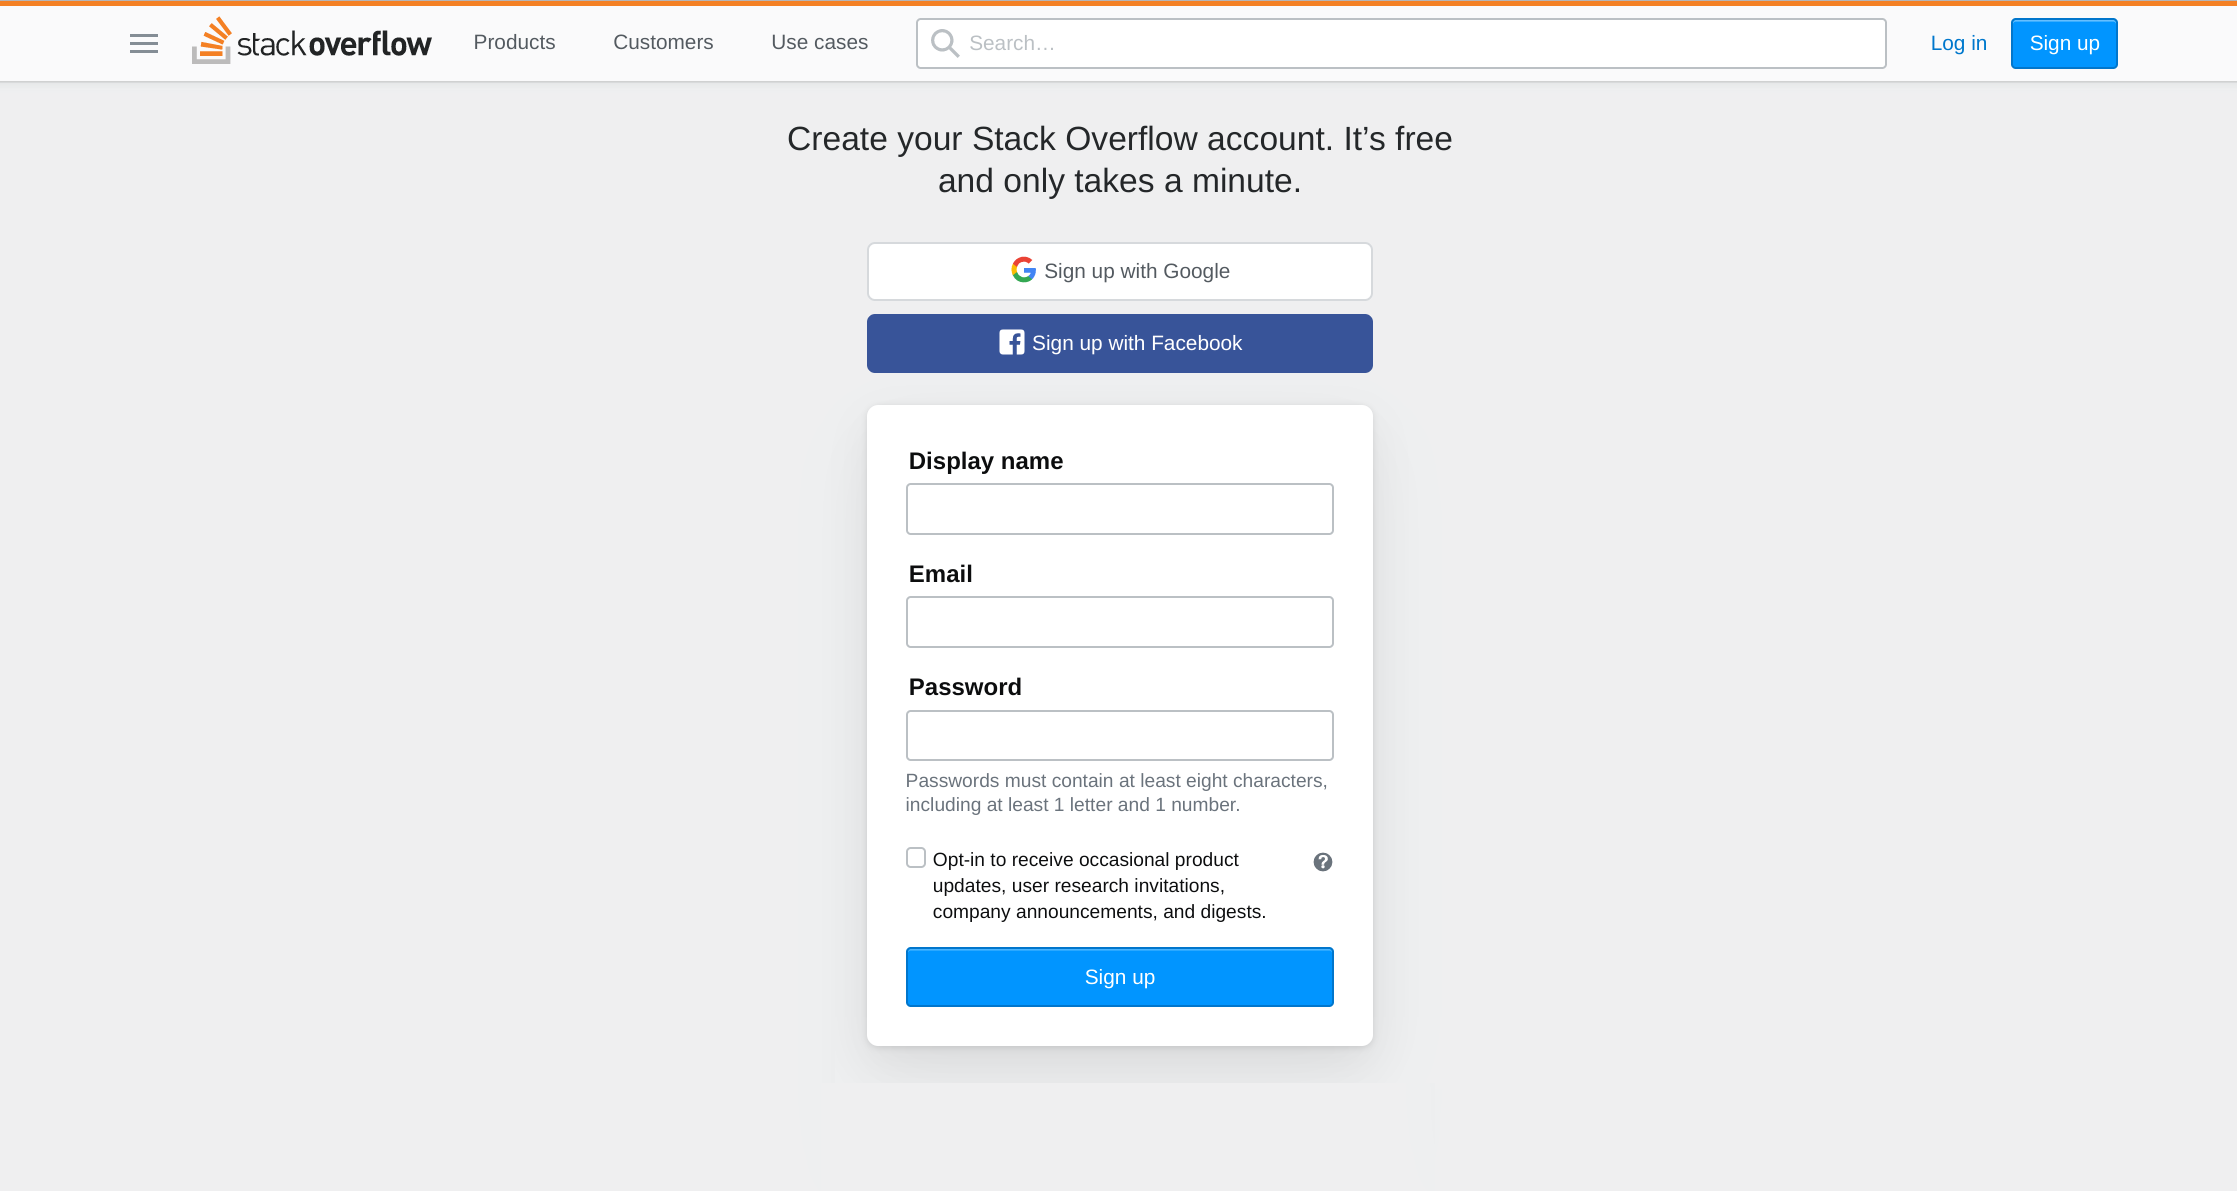
\includegraphics[width=\linewidth]{stackoverflow-signup.png}
\end{columns}
\end{frame}

\begin{frame}{}
\huge
\vspace{1 cm}
\begin{center}
\textcolor{darkblue}{Future of Uproot and Awkward}
\end{center}
\end{frame}

\begin{frame}{Future of Uproot: maintenance}
\Large
\vspace{0.35 cm}
\begin{itemize}\setlength{\itemsep}{0.25 cm}
\item<1-> TTree-writing was the last {\it major} feature planned.
\item<2-> Bugs will be fixed.
\item<3-> Uproot will keep ahead of changes in ROOT I/O.

\vspace{0.05 cm}
\textcolor{gray}{\normalsize (Only one change in ROOT I/O in uproot's two-year existence: \mintinline{c++}{TIOFeatures}.)}

\item<4-> ROOT's future \mintinline{c++}{RNtuple} can probably be handled with semi-independent code, as uproot-methods is now.
\item<5-> ``Uproot 4.0'' will be a transition to Awkward 1.0.
\end{itemize}

\normalsize
\vspace{0.25 cm}
\uncover<6->{\textcolor{gray}{(Apart from TTree-writing, uproot has been in maintenance mode for a year already.)}}
\end{frame}

\begin{frame}{Future of Awkward: consolidation}
\Large
\vspace{0.35 cm}
\begin{itemize}\setlength{\itemsep}{0.25 cm}
\item<1-> Awkward has been tested ``in the wild'' for a year now.
\item<2-> Pure Numpy implementation does some complex (clever!) things to perform jagged operations: no \mintinline{python}{for} loops allowed.

\vspace{0.1 cm}
\begin{itemize}\setlength{\itemsep}{0.2 cm}
\item<3-> \large There are limits to cleverness: many edge cases not handled.
\item<4-> \large Most frequent bugs are due to Numpy usage (e.g.\ \mintinline{python}{numpy.max([])}).
\item<5-> \large Desire to use awkward-arrays in Numba, on GPUs, and in C++ library interfaces leads to duplication; hard to synchronize implementations.
\end{itemize}

\item<6-> Feedback from users revealed some interface mistakes.

\vspace{0.1 cm}
\begin{itemize}\setlength{\itemsep}{0.2 cm}
\item<7-> \large \mintinline{python}{a.cross(b)} versus \mintinline{python}{awkward.cross(a, b)}
\item<8-> \large User-visible \mintinline{python}{JaggedArray} versus \mintinline{python}{ChunkedArray(JaggedArray)}
\end{itemize}
\end{itemize}
\end{frame}

\begin{frame}{}
\huge
\vspace{1 cm}
\begin{center}
\textcolor{darkblue}{Awkward 1.0}
\end{center}
\end{frame}

\begin{frame}{Awkward 1.0 is a {\it rewrite}, improving structure and interface}
\vspace{0.2 cm}
\begin{columns}
\column{1.15\linewidth}
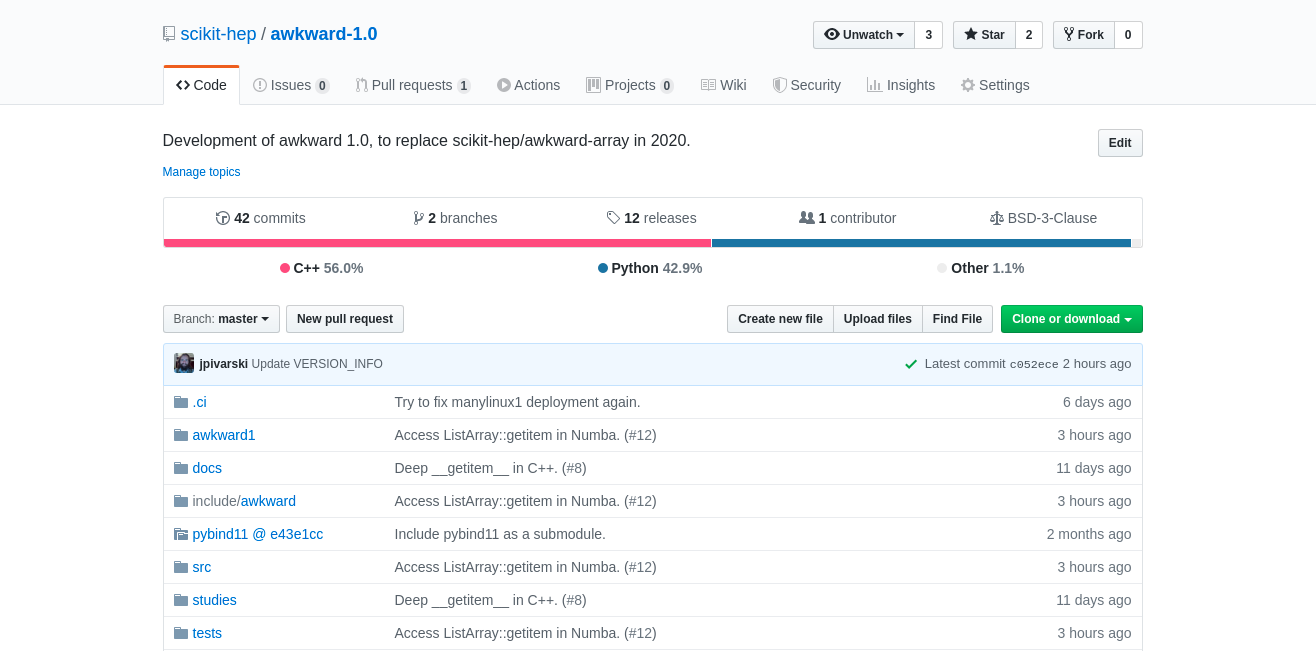
\includegraphics[width=\linewidth]{awkward-1-github.png}
\end{columns}
\end{frame}

\begin{frame}{Layered architecture}
\large
\vspace{0.5 cm}
\begin{columns}
\column{0.5\linewidth}
\vspace{-0.2 cm}

\textcolor{darkblue}{Layer 1:} Python user interface: a single \mintinline{python}{awkward.Array} class.
\vspace{\baselineskip}

\vspace{0.18 cm}
\textcolor{darkblue}{Layer 2:} Structure classes, ``layout''

(e.g.\ \mintinline{python}{ListArray}/\mintinline{python}{RecordArray}).
\vspace{\baselineskip}

\vspace{0.18 cm}
\textcolor{darkblue}{Layer 3:} Memory management, array allocation and ownership; reference counting.
\vspace{\baselineskip}

\vspace{0.18 cm}
\textcolor{darkblue}{Layer 4:} Implementations, where we write \mintinline{python}{for} loops. The only layer that needs to be optimized for speed.

\column{0.5\linewidth}
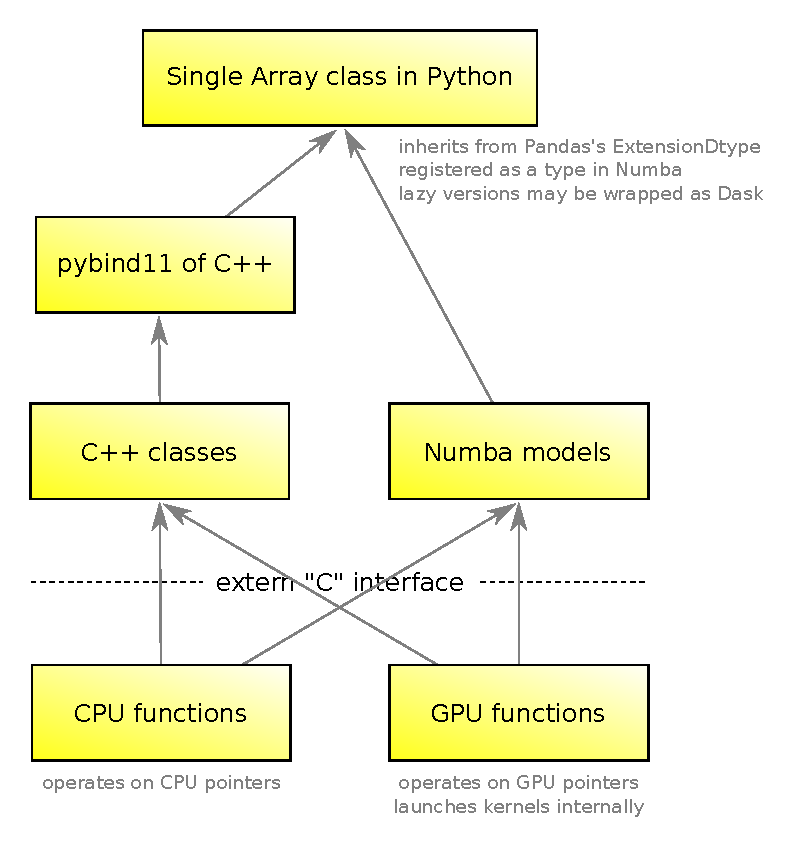
\includegraphics[width=\linewidth]{awkward-1-0-layers.pdf}
\end{columns}
\end{frame}

\begin{frame}[fragile]{Layer 2: pybind11 of C++}
\vspace{0.5 cm}
\hfill\mbox{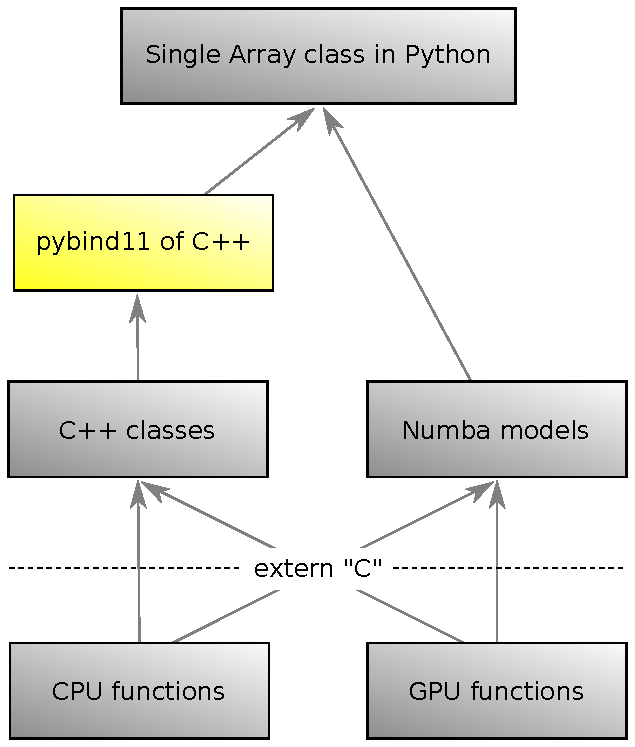
\includegraphics[height=4 cm]{awkward-1-0-layers-mini-pybind11.pdf}\hspace{-0.75 cm}}

\scriptsize
\vspace{-4.45 cm}
\begin{columns}
\column{1.1\linewidth}
\begin{minted}{python}
import numpy
import awkward1

content = awkward1.layout.NumpyArray(numpy.arange(10)*1.1)
listA   = awkward1.layout.ListOffsetArray32(
            awkward1.layout.Index32(numpy.array([0, 3, 3, 5, 6, 10])),
            content)
listB   = awkward1.layout.ListOffsetArray32(
            awkward1.layout.Index32(numpy.array([0, 3, 4, 4, 5])),
            listA)
\end{minted}
\begin{uncoverenv}<2->
\begin{minted}{python}
print(awkward1.tolist(listA))
\end{minted}

\vspace{-0.25 cm}
\begin{Verbatim}[commandchars=\\\{\}]
\textcolor{red}{[[0.0, 1.1, 2.2], [], [3.3, 4.4], [5.5], [6.6, 7.7, 8.8, 9.9]]}
\end{Verbatim}
\end{uncoverenv}
\begin{uncoverenv}<3->
\begin{minted}{python}
print(awkward1.tolist(listB))
\end{minted}

\vspace{-0.25 cm}
\begin{Verbatim}[commandchars=\\\{\}]
\textcolor{red}{[[[0.0, 1.1, 2.2], [], [3.3, 4.4]], [[5.5]], [], [[6.6, 7.7, 8.8, 9.9]]]}
\end{Verbatim}
\end{uncoverenv}
\begin{uncoverenv}<4->
\begin{minted}{python}
print(awkward1.tolist(listB[:, ::-1, ::2]))
\end{minted}

\vspace{-0.25 cm}
\begin{Verbatim}[commandchars=\\\{\}]
\textcolor{red}{[[[3.3], [], [0.0, 2.2]], [[5.5]], [], [[6.6, 8.8]]]}    \textcolor{gray}{(old awkward-array can't do this)}
\end{Verbatim}
\end{uncoverenv}
\begin{uncoverenv}<5->
\begin{minted}{python}
print(awkward1.tolist(listB[[0, 0, -1, -1], [0, -1, 0, -1], 1:-1]))
\end{minted}

\vspace{-0.25 cm}
\begin{Verbatim}[commandchars=\\\{\}]
\textcolor{red}{[[1.1], [], [7.7, 8.8], [7.7, 8.8]]}                     \textcolor{gray}{(mixing fancy and basic indexing)}
\end{Verbatim}
\end{uncoverenv}
\end{columns}
\vspace{1 cm}
\end{frame}

\begin{frame}[fragile]{Layer 3: C++ classes}
\vspace{0.5 cm}
\hfill\mbox{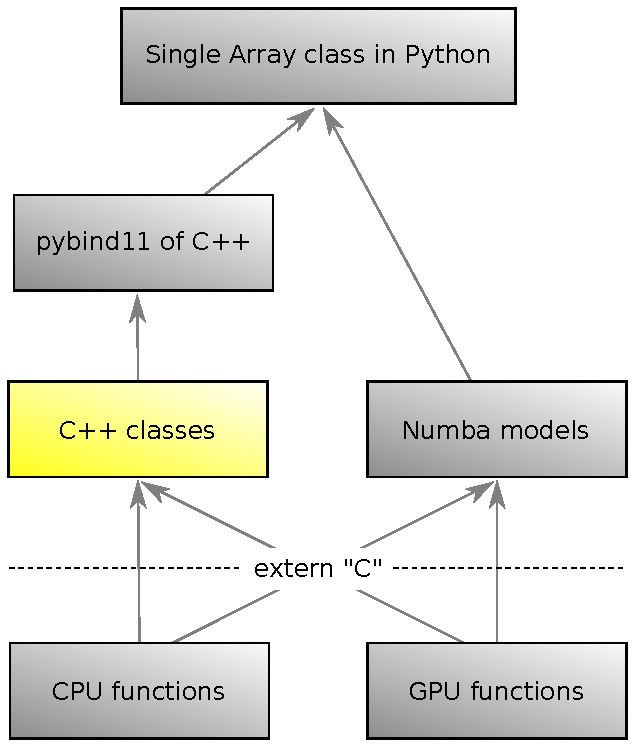
\includegraphics[height=4 cm]{awkward-1-0-layers-mini-cpp.pdf}\hspace{-0.75 cm}}

\scriptsize
\vspace{-4.45 cm}
\begin{columns}
\column{1.1\linewidth}
\begin{minted}{c++}
Index32 offsets(6);
offsets.ptr().get()[0] = 0;    offsets.ptr().get()[3] = 5;
offsets.ptr().get()[1] = 3;    offsets.ptr().get()[4] = 6;
offsets.ptr().get()[2] = 3;    offsets.ptr().get()[5] = 10;

auto raw = new RawArrayOf<double>(Identity::none(), 10);
for (int i = 0;  i < 10;  i++) {
  *raw->borrow(i) = 1.1*i;
}
std::shared_ptr<Content> content(raw);
std::shared_ptr<Content> list(new ListOffsetArray32(Identity::none(),
                                                    offsets, content));
\end{minted}
\begin{uncoverenv}<2->
\begin{minted}{c++}
tostring(list);
\end{minted}

\vspace{-0.25 cm}
\begin{Verbatim}[commandchars=\\\{\}]
\textcolor{red}{"[[0, 1.1, 2.2], [], [3.3, 4.4], [5.5], [6.6, 7.7, 8.8, 9.9]]"}
\end{Verbatim}
\begin{minted}{c++}
tostring(list.get()->getitem_range(1, -1));
\end{minted}

\vspace{-0.25 cm}
\begin{Verbatim}[commandchars=\\\{\}]
\textcolor{red}{"[[], [3.3, 4.4], [5.5]]"}
\end{Verbatim}
\begin{minted}{c++}
tostring(list.get()->getitem(slice(new SliceRange(2, Slice::none(), Slice::none()),
                                   new SliceRange(Slice::none(), Slice::none(), -1))));
\end{minted}

\vspace{-0.25 cm}
\begin{Verbatim}[commandchars=\\\{\}]
\textcolor{red}{"[[4.4, 3.3], [5.5], [9.9, 8.8, 7.7, 6.6]]"}
\end{Verbatim}
\end{uncoverenv}
\end{columns}
\vspace{1 cm}
\end{frame}

\begin{frame}[fragile]{Layer 3: Numba models}
\vspace{0.5 cm}
\hfill\mbox{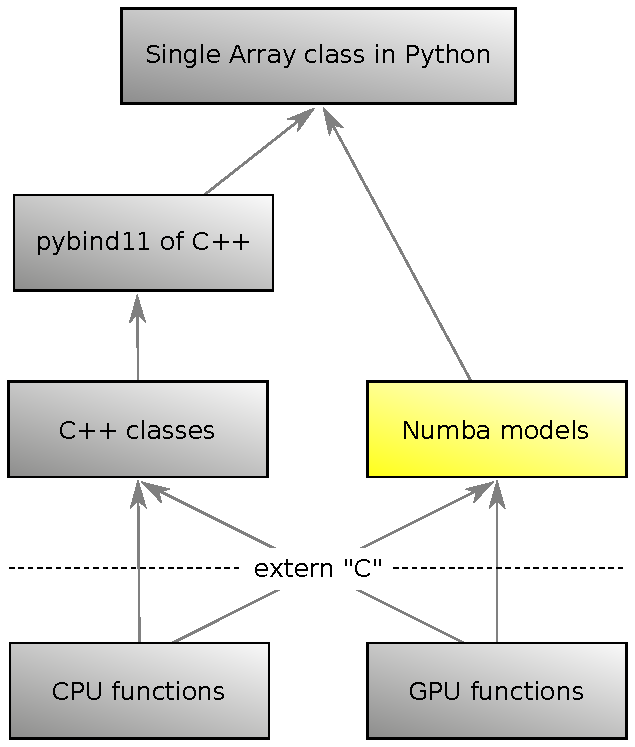
\includegraphics[height=4 cm]{awkward-1-0-layers-mini-numba.pdf}\hspace{-0.75 cm}}

\scriptsize
\vspace{-4.45 cm}
\begin{columns}
\column{1.1\linewidth}
\begin{minted}{python}
import numba

@numba.jit(nopython=True)
def iterate(array):
    out = 0.0
    for subarray in array:               # for loops in a Numba-
        for subsubarray in subarray:     # compiled function are
            for item in subsubarray:     # just as fast as C or C++
                out += item
    return out

print(iterate(listB))
\end{minted}

\vspace{-0.25 cm}
\begin{Verbatim}[commandchars=\\\{\}]
\textcolor{red}{49.5}
\end{Verbatim}
\begin{uncoverenv}<2->
\begin{minted}{python}
@numba.jit(nopython=True)
def slices(array):                       # same slicing works in the compiled environment
    return (array[:, ::-1, ::2],
            array[[0, 0, -1, -1], [0, -1, 0, -1], 1:-1])

one, two = slices(listB)
print(awkward1.tolist(one), awkward1.tolist(two))
\end{minted}

\vspace{-0.25 cm}
\begin{Verbatim}[commandchars=\\\{\}]
\textcolor{red}{[[[3.3], [], [0.0, 2.2]], [[5.5]], [], [[6.6, 8.8]]]}    \textcolor{gray}{(same results as before)}
\textcolor{red}{[[1.1], [], [7.7, 8.8], [7.7, 8.8]]}
\end{Verbatim}
\end{uncoverenv}
\end{columns}
\vspace{1 cm}
\end{frame}

\begin{frame}[fragile]{Layer 4: CPU functions}
\vspace{0.5 cm}
\hfill\mbox{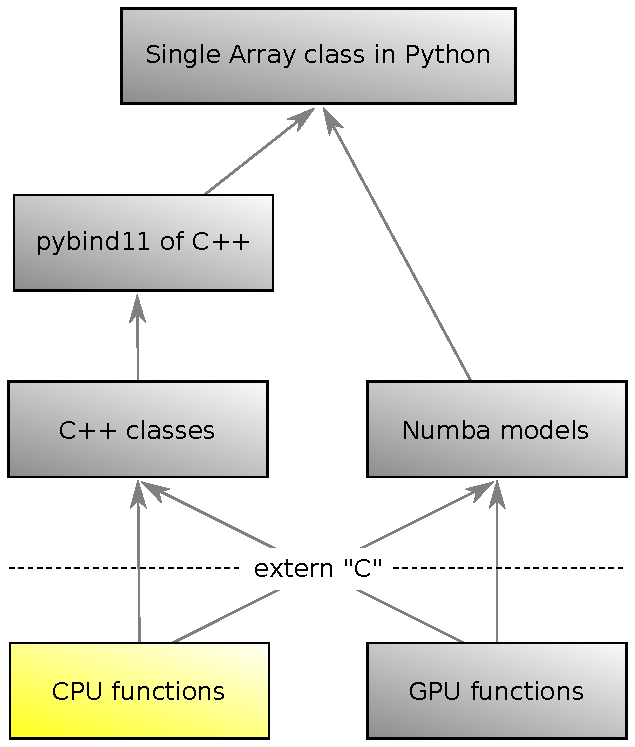
\includegraphics[height=4 cm]{awkward-1-0-layers-mini-cpu.pdf}\hspace{-0.75 cm}}

\scriptsize
\vspace{-4.45 cm}
\begin{columns}
\column{1.1\linewidth}
\begin{uncoverenv}<2->
\begin{minted}{c++}
template <typename C, typename T>
Error awkward_listarray_getitem_next_at(T* tocarry, const C* fromstarts,
          const C* fromstops, int64_t lenstarts, int64_t startsoffset,
          int64_t stopsoffset, int64_t at)
\end{minted}
\end{uncoverenv}

\vspace{-0.35 cm}
\begin{minted}{c++}
{
  for (int64_t i = 0;  i < lenstarts;  i++) {
    int64_t length = fromstops[stopsoffset + i] -
                     fromstarts[startsoffset + i];
    int64_t regular_at = at;
    if (regular_at < 0) {
      regular_at += length;
    }
    if (!(0 <= regular_at  &&  regular_at < length)) {
      return failure("index out of range", i, at);
    }
    tocarry[i] = fromstarts[startsoffset + i] + regular_at;
  }
  return success();
}
\end{minted}

\vspace{-0.35 cm}
\begin{uncoverenv}<3->
\begin{minted}{c++}
extern "C" {
  Error awkward_listarray32_getitem_next_at_64(int64_t* tocarry, const int32_t* fromstarts,
            const int32_t* fromstops, int64_t lenstarts, int64_t startsoffset,
            int64_t stopsoffset, int64_t at);
\end{minted}
\end{uncoverenv}
\end{columns}
\vspace{1 cm}
\end{frame}

\begin{frame}[fragile]{Layer 3: C++ classes}
\vspace{0.5 cm}
\hfill\mbox{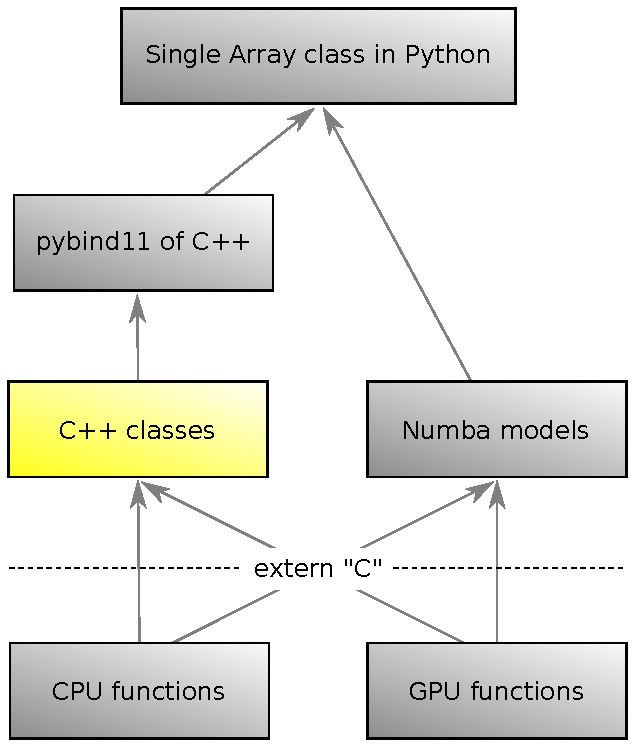
\includegraphics[height=4 cm]{awkward-1-0-layers-mini-cpp.pdf}\hspace{-0.75 cm}}

\scriptsize
\vspace{-4.45 cm}
\begin{columns}
\column{1.1\linewidth}
\begin{minted}{c++}
if (head.get() == nullptr) {
  return shallow_copy();
}

else if (SliceAt* at = dynamic_cast<SliceAt*>(head.get())) {
  std::shared_ptr<SliceItem> nexthead = tail.head();
  Slice nexttail = tail.tail();
  Index64 nextcarry(lenstarts);
  Error err = awkward_listarray32_getitem_next_at_64(
    nextcarry.ptr().get(),
    starts_.ptr().get(),
    stops_.ptr().get(),
    lenstarts,
    starts_.offset(),
    stops_.offset(),
    at->at());
  util::handle_error(err, classname(), id_.get());
  std::shared_ptr<Content> nextcontent = content_.get()->carry(nextcarry);
  return nextcontent.get()->getitem_next(nexthead, nexttail, advanced);
}

else if (SliceRange* range = dynamic_cast<SliceRange*>(head.get())) {
  ...
\end{minted}
\end{columns}
\vspace{1 cm}
\end{frame}

\begin{frame}[fragile]{Layer 3: Numba models}
\vspace{0.5 cm}
\hfill\mbox{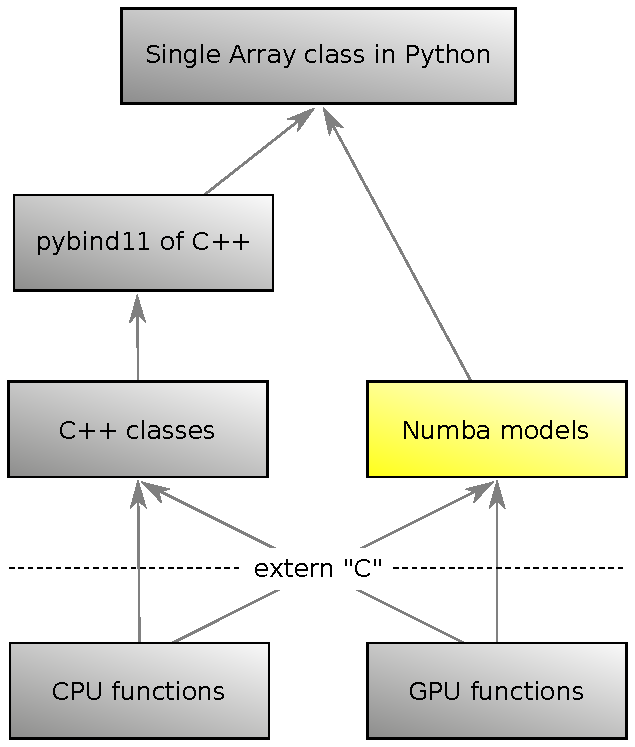
\includegraphics[height=4 cm]{awkward-1-0-layers-mini-numba.pdf}\hspace{-0.75 cm}}

\scriptsize
\vspace{-4.45 cm}
\begin{columns}
\column{1.1\linewidth}
\begin{minted}{python}
if isinstance(headtpe, numba.types.Integer):
  if arraytpe.bitwidth == 64:
    kernel = cpu.kernels.awkward_listarray64_getitem_next_at_64
  elif arraytpe.bitwidth == 32:
    kernel = cpu.kernels.awkward_listarray32_getitem_next_at_64

  nextcarry = util.newindex64(context, builder, numba.int64, lenstarts)
  util.call(context, builder, kernel,
    (util.arrayptr(context, builder, util.index64tpe, nextcarry),
     util.arrayptr(context, builder, arraytpe.startstpe, proxyin.starts),
     util.arrayptr(context, builder, arraytpe.stopstpe, proxyin.stops),
     lenstarts,
     context.get_constant(numba.int64, 0),
     context.get_constant(numba.int64, 0),
     util.cast(context, builder, headtpe, numba.int64, headval)),
    "in {}, indexing error".format(arraytpe.shortname))
  nextcontenttpe = arraytpe.contenttpe.carry()
  nextcontentval = arraytpe.contenttpe.lower_carry(context, builder, arraytpe.contenttpe,
                                           util.index64tpe, proxyin.content, nextcarry)
  return nextcontenttpe.lower_getitem_next(context, builder, nextcontenttpe, tailtpe,
                                           nextcontentval, tailval, advanced)
elif isinstance(headtpe, numba.types.SliceType):
  ...
\end{minted}
\end{columns}
\vspace{1 cm}
\end{frame}

\begin{frame}{Still following the array-at-a-time approach}
\large
\vspace{1 cm}
\begin{columns}
\column{1.07\linewidth}
Slow Python has been replaced by slow C++ (dynamic dispatch, runtime type-checks).

\vspace{0.75 cm}
But only $\mathcal{O}(\mbox{depth of type})$ operations are performed in C++; $\mathcal{O}(\mbox{number of events})$ operations are performed in single-pass cpu-functions.
\end{columns}

\begin{center}
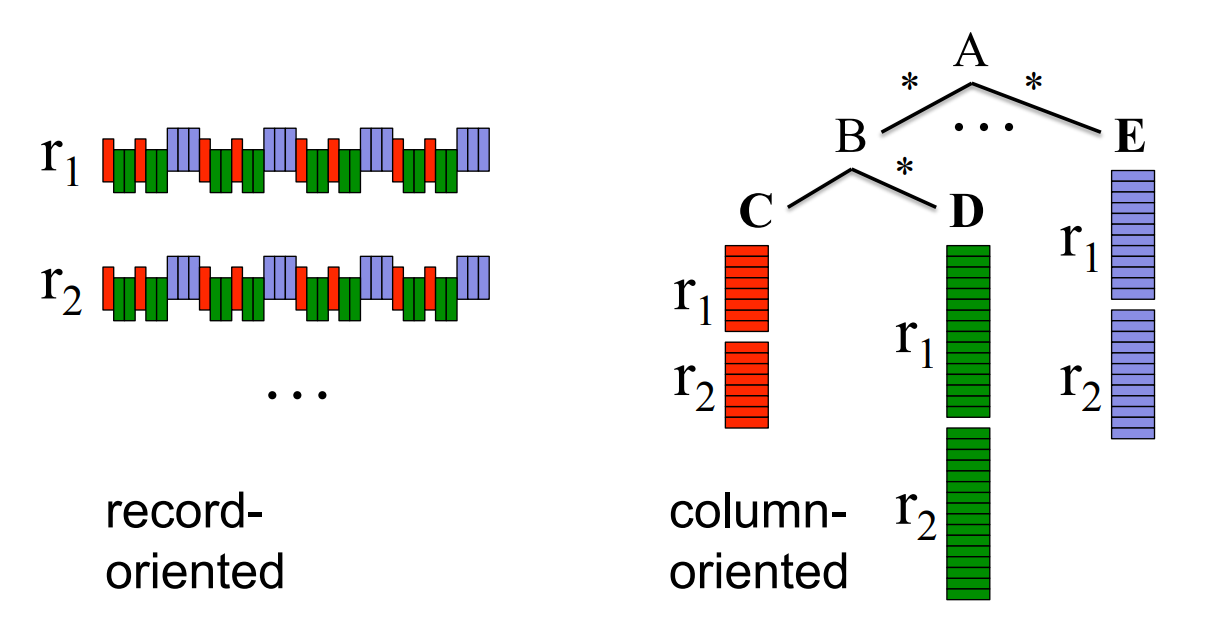
\includegraphics[width=0.5\linewidth]{google-dremel-fig1.png}
\end{center}
\end{frame}

\begin{frame}{Deliverables}
\large
\vspace{0.75 cm}
Compilable by CMake (for pure C++) or \mintinline{bash}{python setup.py install}.

\vspace{0.5 cm}
\begin{description}\setlength{\itemsep}{0.5 cm}
\item[cpu-kernels.so] suite of Layer 4 functions with an \mintinline{c++}{extern "C"} interface, which can be accessed by any language (notably C++ and Numba).

\item[libawkward.so] library of Layer 3 classes that can be used in any C++ project.

\item[\hspace{0.75 cm}awkward1] Python library: Layer 1 (user interface), Layer 2 (extension module), and Layer 3 (Numba extensions, if Numba is installed).
\end{description}

\vspace{0.75 cm}
\textcolor{blue}{\normalsize \url{https://pypi.org/project/awkward1/\#files}} hosts 29 binary wheels and 1 source package; most users will \mintinline{bash}{pip install} without compiling.
\end{frame}

\begin{frame}{}
\huge
\vspace{1 cm}
\begin{center}
\textcolor{darkblue}{Mathematical aspects}
\end{center}
\end{frame}

\begin{frame}[fragile]{Functional programming for arrays}
\large
\vspace{0.4 cm}
Arrays are functions:

\vspace{-0.45 cm}
\[ \mintinline{python}{array}: [0, n) \to \mintinline{python}{dtype} \]

\vspace{0.15 cm}
such that \mintinline{python}{array[i]} for integer \mintinline{python}{i} is a function call.

\vspace{0.5 cm}
\begin{uncoverenv}<2->
Indexing by an integer array is functional composition:

\vspace{-0.5 cm}
\[ \mintinline{python}{ints}: [0, m) \to [0, n) \hspace{1 cm}\Rightarrow\hspace{1 cm} \mintinline{python}{array[ints]}: [0, m) \to \mintinline{python}{dtype} \]
\end{uncoverenv}

\vspace{-0.35 cm}
\begin{uncoverenv}<3->
So if \mintinline{python}{f} and \mintinline{python}{g} are $\mathbb{Z}^{\mbox{\tiny $\ge\hspace{-0.05 cm}0$}} \to \mathbb{Z}^{\mbox{\tiny $\ge\hspace{-0.05 cm}0$}}$ functions and we sample them as \mintinline{python}{F} and \mintinline{python}{G},
\normalsize
\begin{minted}{python}
    F   = numpy.array([f(i)    for i in range(...)])
    G   = numpy.array([g(i)    for i in range(...)])
    GoF = numpy.array([g(f(i)) for i in range(...)])
\end{minted}

\large
\vspace{0.1 cm}
then \fbox{$\mintinline{python}{G[F]} = \mintinline{python}{GoF}$}.
\end{uncoverenv}

\vspace{0.5 cm}
\begin{uncoverenv}<4->
Functional composition is associative: if \mintinline{python}{H} is any array, \fbox{$\mintinline{python}{H[G][F]} = \mintinline{python}{H[G[F]]}$}.
\end{uncoverenv}
\end{frame}

\begin{frame}{Associativity of integer-array indexing is a very useful feature}
\vspace{0.2 cm}
\begin{columns}
\column{0.485\linewidth}
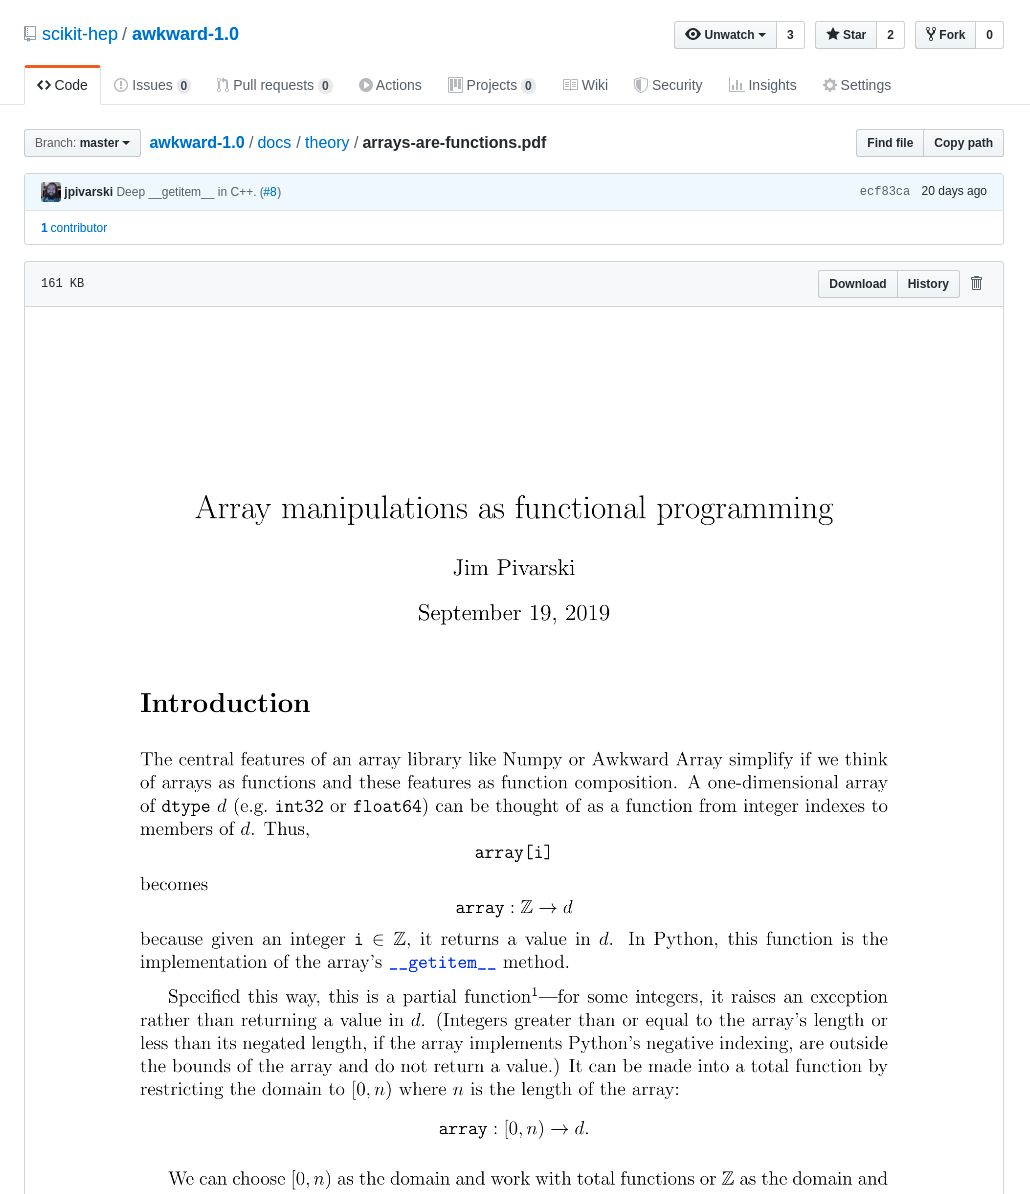
\includegraphics[width=\linewidth]{arrays-as-functions-paper.png}

\column{0.5\linewidth}
\small
\textcolor{blue}{\url{https://github.com/scikit-hep/awkward-1.0/blob/master/docs/theory/arrays-are-functions.pdf}}

\large
\vspace{1 cm}
Used throughout \mintinline{c++}{getitem_next} to ``carry'' information from one level of recursion to the next, in analogy with carrying digits in longhand addition.
\end{columns}
\end{frame}

\begin{frame}{}
\huge
\vspace{1 cm}
\begin{center}
\textcolor{darkblue}{Pandas-style indexing}
\end{center}
\end{frame}

\begin{frame}[fragile]{Indexing distinguishes Numpy from Pandas and xarray}
\large
\vspace{0.6 cm}
\begin{columns}
\column{1.5 cm}

\includegraphics[height=2 cm]{numpy-logo.png}

\column{0.5 cm}
\centering \huge vs.

\column{4.5 cm}

\includegraphics[height=2 cm]{pandas-logo.png}\hspace{0.5 cm}
\includegraphics[height=2 cm]{xarray-logo.png}
\end{columns}

\vspace{0.5 cm}
\begin{columns}
\column{1.03\linewidth}
Awkward 1.0 operations will optionally pass around an \mintinline{c++}{Identity}, an extra array that attaches permanent coordinates to each number, list, and record in the data.

\vspace{0.25 cm}
\begin{uncoverenv}<2->
Good for error messages\ldots

\small
\begin{minted}{python}
>>> dataset.setid()   # generate Identities
>>> primary_jet_for_muon = dataset[:, "muons", :, "jets", 0]
\end{minted}

\vspace{-0.5 cm}
\begin{onlyenv}<-2>
\begin{Verbatim}[commandchars=\\\{\}]
Traceback (most recent call last):
  File "<stdin>", line 2, in <module>
ValueError: in ListArray32 at id[10374, "muons", 1, "jets"] attempting
            to get 0, index out of range
\end{Verbatim}
\end{onlyenv}\begin{onlyenv}<3>
\begin{Verbatim}[commandchars=\\\{\}]
Traceback (most recent call last):
  File "<stdin>", line 2, in <module>
ValueError: in ListArray32 \textcolor{darkgreen2}{\underline{\tt{}at id[10374, "muons", 1, "jets"]}} attempting
            to get 0, index out of range
\end{Verbatim}
\end{onlyenv}
\end{uncoverenv}
\end{columns}
\end{frame}

\begin{frame}[fragile]{\ldots but it was motivated by investigations into set-based languages}
\vspace{0.1 cm}
\begin{center}
\fbox{\textcolor{blue}{\url{https://github.com/jpivarski/PartiQL}}}
\end{center}

\vspace{-0.25 cm}
\begin{columns}
\column{1.02\linewidth}
\scriptsize
\begin{Verbatim}[commandchars=\\\{\}]
\textcolor{gray}{# For events with at least three leptons (electrons or muons) and a same-flavor}
\textcolor{gray}{# opposite-sign lepton pair, find the same-flavor opposite-sign lepton pair with a}
\textcolor{gray}{# mass closest to 91.2 GeV; make a histogram of the pT of the leading other lepton.}
\end{Verbatim}

\small
\vspace{-0.25 cm}
\begin{Verbatim}[commandchars=\\\{\}]
leptons = electrons \textcolor{darkgreen}{\textbf{union}} muons
\end{Verbatim}

\vspace{-0.45 cm}
\begin{Verbatim}[commandchars=\\\{\}]
\textcolor{darkgreen}{\textbf{cut}} \textcolor{blue}{count}(leptons) >= \textcolor{darkorange}{3} \textcolor{darkgreen}{\textbf{named}} \textcolor{darkorange}{"three_leptons"} \{
    Z = electrons \textcolor{darkgreen}{\textbf{as}} (lep1, lep2) \textcolor{darkgreen}{\textbf{union}} muons \textcolor{darkgreen}{\textbf{as}} (lep1, lep2)
            \textcolor{darkgreen}{\textbf{where}} lep1\textcolor{blue}{.charge} != lep2\textcolor{blue}{.charge}
            \textcolor{darkgreen}{\textbf{min by}} \textcolor{blue}{abs}(\textcolor{blue}{mass}(lep1, lep2) - \textcolor{darkorange}{91.2})
\end{Verbatim}

\vspace{-0.45 cm}
\begin{Verbatim}[commandchars=\\\{\}]
    third = leptons \textcolor{darkgreen}{\textbf{except}} [Z\textcolor{blue}{.lep1}, Z\textcolor{blue}{.lep2}] \textcolor{darkgreen}{\textbf{max by}} pt
    \textcolor{darkgreen}{\textbf{hist}} third.pt \textcolor{darkgreen}{\textbf{by}} \textcolor{blue}{regular}(\textcolor{darkorange}{100}, \textcolor{darkorange}{0}, \textcolor{darkorange}{250}) \textcolor{darkgreen}{\textbf{named}} \textcolor{darkorange}{"third_pt"}
\}
\end{Verbatim}

\large
\fbox{\begin{minipage}{\linewidth}
An \mintinline{c++}{Identity} (surrogate-key index) is needed to define set operations like \textcolor{darkgreen}{\tt\textbf{join}}, \textcolor{darkgreen}{\tt\textbf{cross}}, \textcolor{darkgreen}{\tt\textbf{union}}, and \textcolor{darkgreen}{\tt\textbf{except}} such that particles are never duplicated.
\end{minipage}}
\end{columns}
\end{frame}

\begin{frame}{Multi-paradigm arrays}
\large
\vspace{0.75 cm}
With a dataset in Awkward form (from TTrees, RNtuples, Arrow\ldots), we want to

\vspace{0.25 cm}
\begin{itemize}\setlength{\itemsep}{0.25 cm}
\item<2-> perform Numpy-like slicing, reduction, and vectorized operations,
\item<3-> enter a compiled Numba function for imperative code in Python,
\item<4-> pass to/from a C++ library (e.g.\ jagged array of Lorentz vectors to FastJet),
\item<5-> compute combinatorics with a HEP-specific domain specific language,
\end{itemize}

\vspace{0.25 cm}
\uncover<6->{\underline{interchangeably}.}

\vspace{0.5 cm}
\begin{center}
\uncover<7->{\textcolor{darkorange}{\bf Awkward 1.0 is intended as a solid foundation for that future.}}
\end{center}
\end{frame}

\begin{frame}{When can I try it?}
\Large
\begin{center}
\textcolor{darkblue}{Nowish:} it is in a testable state \textcolor{gray}{(for Coffea and thrill-seekers)}.

\vspace{1 cm}
Will be minimally usable for physics analysis in ``early 2020.''

\vspace{1 cm}
\end{center}

Start an {\normalsize \mintinline{python}{import awkward}} $\to$ {\normalsize \mintinline{python}{import awkward0}} \\
\phantom{Start an} {\normalsize \mintinline{python}{import awkward1}} $\to$ {\normalsize \mintinline{python}{import awkward}} transition by spring.
\end{frame}

\begin{frame}{}
\vspace{-0.02 cm}
\begin{columns}
\column{1.2\linewidth}
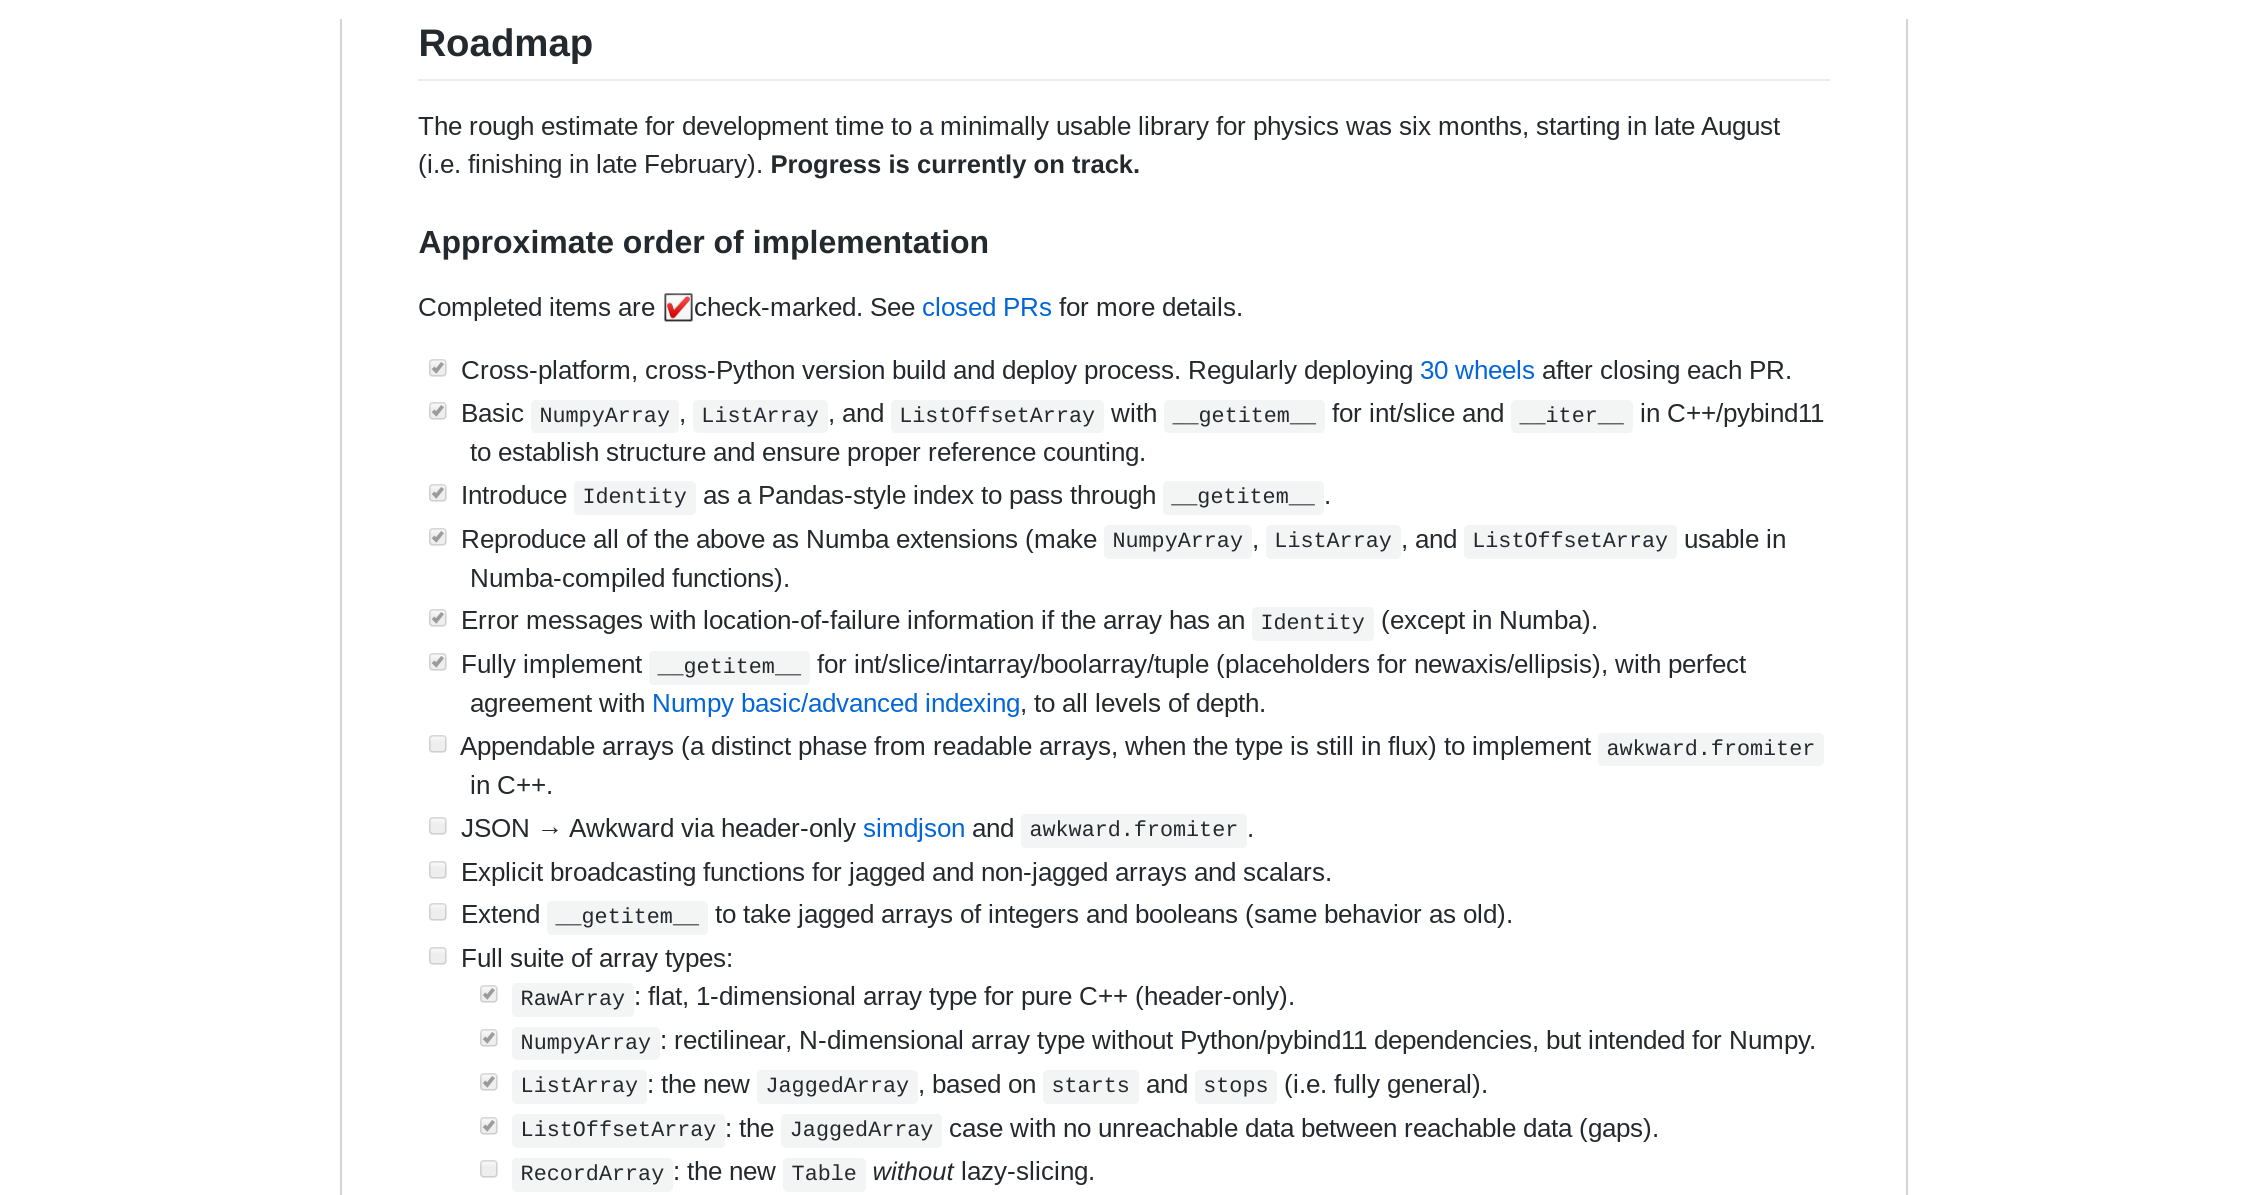
\includegraphics[width=\linewidth]{awkward-roadmap.png}
\end{columns}
\end{frame}

\begin{frame}{Did you get a StackOverflow account?}
\vspace{0.15 cm}
\begin{columns}
\column{1.2\linewidth}
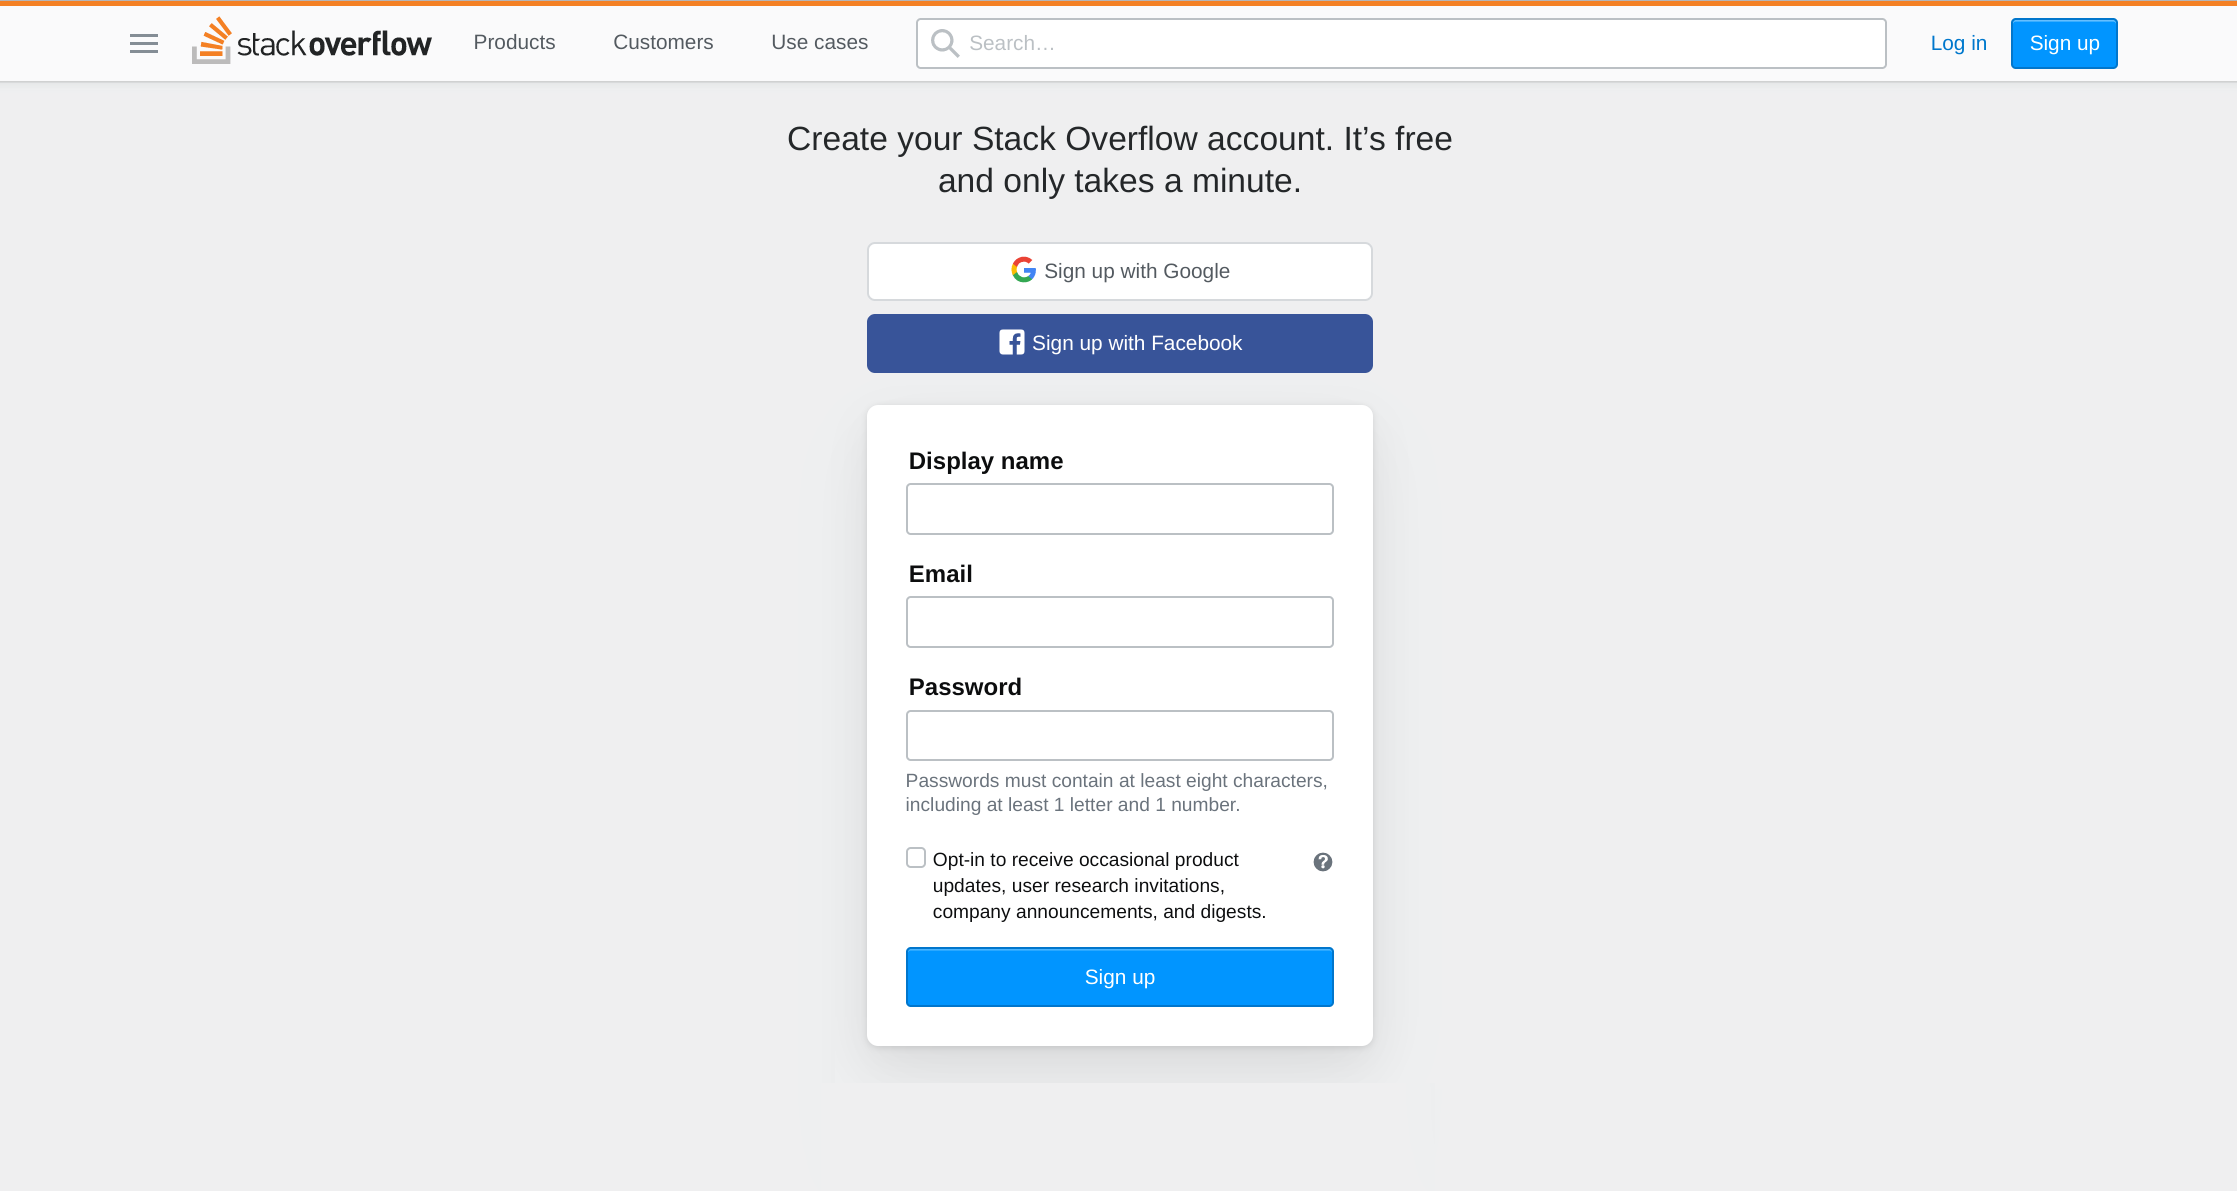
\includegraphics[width=\linewidth]{stackoverflow-signup.png}
\end{columns}
\end{frame}

\end{document}
